\documentclass{article}
\usepackage{tikz, comment}
\usepackage{pifont}
\usepackage{fontspec}
\usetikzlibrary{arrows, decorations.markings, decorations.pathreplacing}
\begin{comment}
:Title: Not defined yet
:Tags: pi;;area using polar coordinates, polar integral formula ;moment;cosine, cos ;polar form of a complex number
:Prob: 0.4136;0.4077;0.4011;0.396;0.3847
:Author: Prof.Hu Ji-shan, HKUST
:Slug: No name yet

Description Here.........
\end{comment}
\begin{document}\centering

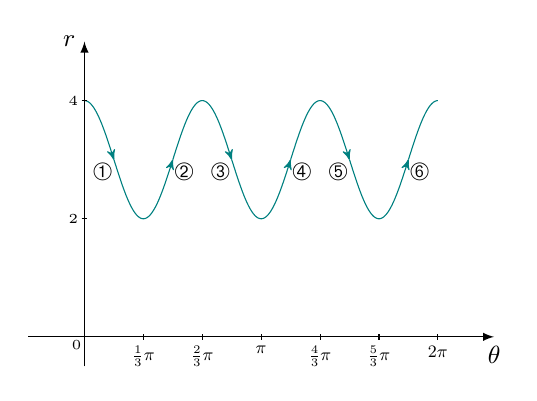
\begin{tikzpicture}[>=latex,xscale=.5/0.7, yscale=.5*1.5][font=\sf\small]

\draw[->, >=stealth', teal, samples=150, smooth, domain=0:pi/6, variable=\t]
plot ({\t}, {3+cos(3*\t r)}) -- ({pi/6}, {3+cos(3*(pi/6) r)});

\draw[->, >=stealth', teal, samples=150, smooth, domain=pi/6:3*pi/6, variable=\t]
plot ({\t}, {3+cos(3*\t r)}) -- ({3*pi/6}, {3+cos(3*(3*pi/6) r)});

\draw[->, >=stealth', teal, samples=150, smooth, domain=3*pi/6:5*pi/6, variable=\t]
plot ({\t}, {3+cos(3*\t r)}) -- ({5*pi/6}, {3+cos(3*(5*pi/6) r)});

\draw[->, >=stealth', teal, samples=150, smooth, domain=5*pi/6:7*pi/6, variable=\t]
plot ({\t}, {3+cos(3*\t r)}) -- ({7*pi/6}, {3+cos(3*(7*pi/6) r)});

\draw[->, >=stealth', teal, samples=150, smooth, domain=7*pi/6:9*pi/6, variable=\t]
plot ({\t}, {3+cos(3*\t r)}) -- ({9*pi/6}, {3+cos(3*(9*pi/6) r)});

\draw[->, >=stealth', teal, samples=150, smooth, domain=9*pi/6:11*pi/6, variable=\t]
plot ({\t}, {3+cos(3*\t r)}) -- ({11*pi/6}, {3+cos(3*(11*pi/6) r)});

\draw[teal, samples=150, smooth, domain=11*pi/6:2*pi, variable=\t]
plot ({\t}, {3+cos(3*\t r)});

%\draw[xstep=1cm,ystep=1cm,color=gray!80] (0, -1) grid (8, 8);
\foreach \x in {}
\draw (\x,2pt/6) -- (\x,-2pt/6)
node[anchor=north] {\tiny$\x$}
;
\draw ({1*pi/3},2pt/1.5) -- ({1*pi/3},-2pt/1.5)node[anchor=north, xshift=0, scale=0.7] {$\frac{1}{3}\pi$};
\draw ({2*pi/3},2pt/1.5) -- ({2*pi/3},-2pt/1.5)node[anchor=north, xshift=0, scale=0.7] {$\frac{2}{3}\pi$};
\draw ({pi},2pt/1.5) -- ({pi},-2pt/1.5)node[anchor= north, xshift=0, scale=0.7] {$\pi$};
\draw ({4*pi/3},2pt/1.5) -- ({4*pi/3},-2pt/1.5)node[anchor=north, xshift=0, scale=0.7] {$\frac{4}{3}\pi$};
\draw ({5*pi/3},2pt/1.5) -- ({5*pi/3},-2pt/1.5)node[anchor=north, xshift=0, scale=0.7] {$\frac{5}{3}\pi$};
\draw ({2*pi},2pt/1.5) -- ({2*pi},-2pt/1.5)node[anchor= north, xshift=0, scale=0.7] {$2\pi$};

\foreach \x in {}
\draw (\x,2pt*1.5) -- (\x,-2pt*1.5)
node[anchor=south] {\tiny$\x$}
;
\foreach \y in {2,4}
\draw (-2pt*0.7,\y) -- (2pt*0.7,\y)
node[anchor=east] {\tiny $\y$}
;

\draw[->] (-1, 0) -- ({2*pi+1}, 0)node[below] {\small $\theta$} ;
\draw[->] (0, -0.5) -- (0, 5)node[left] {\small $r$} ;

\node at ({1*pi/6 -0.2}, 2.8) {\ding{192}};
\node at ({1*pi/6+2*pi/6+0.2}, 2.8) {\ding{193}};
\node at ({1*pi/6+4*pi/6-0.2}, 2.8) {\ding{194}};
\node at ({1*pi/6+6*pi/6+0.2}, 2.8) {\ding{195}};
\node at ({1*pi/6+8*pi/6-0.2}, 2.8) {\ding{196}};
\node at ({1*pi/6+10*pi/6+0.2}, 2.8) {\ding{197}};

\node at (-0.2*0.7, -0.2/1.5) {\tiny$0$};

\end{tikzpicture}\hskip0.5cm
\end{document}